\documentclass{beamer}
\usepackage[utf8]{inputenc}

\usetheme{Madrid}
\usecolortheme{default}
\usepackage{amsmath,amssymb,amsfonts,amsthm}
\usepackage{txfonts}
\usepackage{tkz-euclide}
\usepackage{listings}
\usepackage{adjustbox}
\usepackage{array}
\usepackage{tabularx}
\usepackage{gvv}
\usepackage{lmodern}
\usepackage{circuitikz}
\usepackage{tikz}
\usepackage{graphicx}

\setbeamertemplate{page number in head/foot}[totalframenumber]

\usepackage{tcolorbox}
\tcbuselibrary{minted,breakable,xparse,skins}



\definecolor{bg}{gray}{0.95}
\DeclareTCBListing{mintedbox}{O{}m!O{}}{%
  breakable=true,
  listing engine=minted,
  listing only,
  minted language=#2,
  minted style=default,
  minted options={%
    linenos,
    gobble=0,
    breaklines=true,
    breakafter=,,
    fontsize=\small,
    numbersep=8pt,
    #1},
  boxsep=0pt,
  left skip=0pt,
  right skip=0pt,
  left=25pt,
  right=0pt,
  top=3pt,
  bottom=3pt,
  arc=5pt,
  leftrule=0pt,
  rightrule=0pt,
  bottomrule=2pt,
  toprule=2pt,
  colback=bg,
  colframe=orange!70,
  enhanced,
  overlay={%
    \begin{tcbclipinterior}
    \fill[orange!20!white] (frame.south west) rectangle ([xshift=20pt]frame.north west);
    \end{tcbclipinterior}},
  #3,
}
\lstset{
    language=C,
    basicstyle=\ttfamily\small,
    keywordstyle=\color{blue},
    stringstyle=\color{orange},
    commentstyle=\color{green!60!black},
    numbers=left,
    numberstyle=\tiny\color{gray},
    breaklines=true,
    showstringspaces=false,
}
%------------------------------------------------------------
%This block of code defines the information to appear in the
%Title page
\title %optional
{4.7.41}
\date{September 20, 2025}
%\subtitle{A short story}

\author % (optional)
{Sai Hasini  - EE25BTECH11044}




\begin{document}

% --- Frame: Problem Statement ---
\begin{frame}{Problem}
\begin{block}{Question}
Find the distance of the point
\[
\vec{P} = \begin{bmatrix} 2 \\ 4 \\ -1 \end{bmatrix}
\]
from the line
\[
\frac{x+5}{1} = \frac{y+3}{4} = \frac{z-6}{-9}.
\]
\end{block}
\end{frame}
\begin{frame}{Solution (1/3)}
The distance formula using projection matrices is
\begin{equation}
d = \Big\|\Big(I-\frac{\vec m \vec m^T}{\vec m^T \vec m}\Big)(\vec p - \vec a)\Big\|.
\label{eq:dist-formula}
\end{equation}
Let
\begin{equation}
\vec w = \vec p - \vec a =
\begin{bmatrix}7\\7\\-7\end{bmatrix}.
\label{eq:w-def}
\end{equation}
\end{frame}

\begin{frame}{Solution (2/3)}
Compute
\begin{equation}
\vec m^T \vec m = 1^2+4^2+(-9)^2 = 98,
\label{eq:m-norm}
\end{equation}
\begin{equation}
\vec m^T \vec w = 1\cdot7 + 4\cdot7 + (-9)(-7) = 98.
\label{eq:m-w-dot}
\end{equation}
So
\begin{equation}
(I-P)\vec w = \vec w - \frac{\vec m^T \vec w}{\vec m^T \vec m}\vec m
= \begin{bmatrix}7\\7\\-7\end{bmatrix} -
\begin{bmatrix}1\\4\\-9\end{bmatrix}.
\label{eq:ipw}
\end{equation}
\end{frame}

\begin{frame}{Solution (3/3)}
\begin{equation}
(I-P)\vec w = \begin{bmatrix}6\\3\\2\end{bmatrix}.
\label{eq:ipw-result}
\end{equation}
Therefore,
\begin{equation}
d = \sqrt{6^2+3^2+2^2} = \sqrt{49} = 7.
\label{eq:final-d}
\end{equation}

\[
\boxed{d=7}
\]
\end{frame}

% ------------------- C CODE -------------------
\begin{frame}[fragile]{C Code (1/3)}
\begin{lstlisting}[language=C]
#include <stdio.h>
#include <math.h>

// Function to compute squared norm of a vector
double norm_sq(double v[3]) {
    return v[0]*v[0] + v[1]*v[1] + v[2]*v[2];
}

// Function to compute dot product
double dot(double v1[3], double v2[3]) {
    return v1[0]*v2[0] + v1[1]*v2[1] + v1[2]*v2[2];
}
\end{lstlisting}
\end{frame}

\begin{frame}[fragile]{C Code (2/3)}
\begin{lstlisting}[language=C]
int main() {
    // Point p
    double p[3] = {2, 4, -1};
    // Point a on line
    double a[3] = {-5, -3, 6};
    // Direction vector of line
    double m[3] = {1, 4, -9};
    
    // Compute w = p - a
    double w[3];
    for (int i = 0; i < 3; i++) {
        w[i] = p[i] - a[i];
    }
\end{lstlisting}
\end{frame}

\begin{frame}[fragile]{C Code (3/3)}
\begin{lstlisting}[language=C]
    // Compute distance
    double d2 = norm_sq(w) - 
               (dot(m, w) * dot(m, w)) / norm_sq(m);
    double d = sqrt(d2);

    printf("Distance from point to line = %.2f\n", d);
    return 0;
}
\end{lstlisting}
\end{frame}

% --- Frame 1 ---
\begin{frame}[fragile]{Python(1/3)}
\begin{lstlisting}[language=Python]
import ctypes
import numpy as np
import matplotlib.pyplot as plt

# Load shared library
lib = ctypes.CDLL("./libdistance.so")

# Define argument and return types
lib.distance_point_line.argtypes = [
    ctypes.POINTER(ctypes.c_double),
    ctypes.POINTER(ctypes.c_double),
    ctypes.POINTER(ctypes.c_double)
]
lib.distance_point_line.restype = ctypes.c_double
\end{lstlisting}
\end{frame}

% --- Frame 2 ---
\begin{frame}[fragile]{Python(2/3)}
\begin{lstlisting}[language=Python]
# Define arrays
p = np.array([2.0, 4.0, -1.0], dtype=np.double)
a = np.array([-5.0, -3.0, 6.0], dtype=np.double)
m = np.array([1.0, 4.0, -9.0], dtype=np.double)

# Call C function
d = lib.distance_point_line(
    p.ctypes.data_as(ctypes.POINTER(ctypes.c_double)),
    a.ctypes.data_as(ctypes.POINTER(ctypes.c_double)),
    m.ctypes.data_as(ctypes.POINTER(ctypes.c_double))
)

print(f"Distance from point to line = {d:.2f}")
# Projection of p onto line
w = p - a
proj = (np.dot(m, w) / np.dot(m, m)) * m
foot = a + proj
\end{lstlisting}
\end{frame}

% --- Frame 3 ---
\begin{frame}[fragile]{Python(3/3)}
\begin{lstlisting}[language=Python]
# Line points
t_vals = np.linspace(-2, 2, 100)
line_points = np.array([a + t*m for t in t_vals])

# Plot in 3D
fig = plt.figure(figsize=(8,6))
ax = fig.add_subplot(111, projection='3d')

ax.plot(line_points[:,0], line_points[:,1], line_points[:,2],
        'b', label="Line")
ax.scatter(p[0], p[1], p[2], color='r', s=50, label="Point P")
ax.plot([p[0], foot[0]], [p[1], foot[1]], [p[2], foot[2]],
        'r--', label="Perpendicular")
ax.scatter(foot[0], foot[1], foot[2],
           color='k', s=60, marker='x', label="Foot")

ax.legend()
plt.show()
\end{lstlisting}
\end{frame}



% --- Frame 6: Plot ---
\begin{frame}{Plot}
\centering
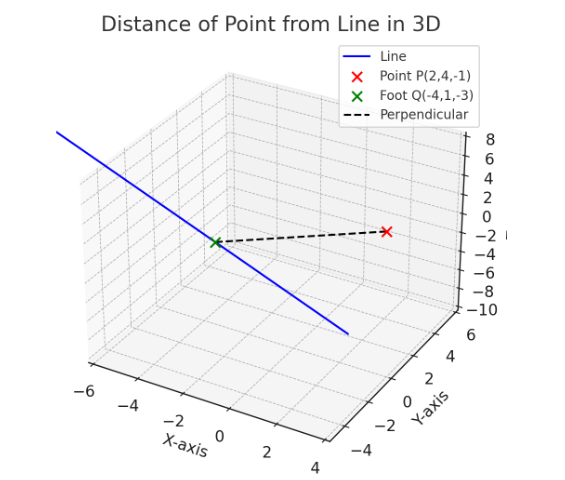
\includegraphics[width=0.8\columnwidth]{figs/plot7.png}
\end{frame}

\end{document}
